As discussed in Chapters \ref{ch:CBCSearches} and \ref{ch:instrumentalDetchar}, the data at the 
output of the LIGO interferometers contain non-Gaussian, transient noise artifacts. 
Chapter \ref{ch:instrumentalDetchar}, \ref{ch:IMCUpconversion}, and \ref{ch:ODC} detail the efforts 
that have been made to understand and remove transient noise in the LIGO interferometers. 
When it was possible, transient noise sources were repaired at the source and the noise was not 
able to impact the output of astrophysical searches. Unfortunately, this is not always possible. 
If a source of transient noise can't be repaired, the noisy data will be processed by astrophysical
search pipelines. 

Transient noise artifacts are 
known to cause loud events at the output of astrophysical searches for gravitational waves, which 
manfiest as a tail in the re-weighted SNR distribution as seen in Figure \ref{subfig:l1-newsnr-hist}. 
The data that comprise this tail of loudest events are the primary target of data quality 
investigations, such as those discussed in Chapter \ref{ch:instrumentalDetchar}. 
If the noise sources can be linked to a 
systematic instrumental cause or a period of highly irregular instrumental performance, 
they can be flagged and removed from the analysis in the form of a 
data quality veto.

It is important to note that data quality vetoes are produced for all analysis time based
on systematic instrumental conditions without any regard for the presence of gravitational wave
signals. All data are treated equally; the removal of data with excess noise has the ability to
remove real gravitational wave signals as well as background events.
There are two types of vetoes implemented in the PyCBC search: category 1 and
category 2.

\section{Veto categories}

Category 1 (CAT1) vetoes are intended to mark times when significant instrumental issues are present
and the data should not be used in any analysis. CAT1 flags often indicate time
when the character of the data has drastically changed and should not be combined
with noise estimations from times of nominal performance.
An example of this from O1 is an electronics failure that dramatically changes the character of the
background noise and creates noise transients at a very high rate.
As such, CAT1 vetoes remove time at the input to the PyCBC search pipeline. This ensures that
severely problematic data are not used for background noise estimations and that no triggers will be
generated at these times.

Category 2 (CAT2) vetoes are intended to mark short, noisy times that
that should not be treated as clean data. CAT2 flags are often
used to flag transients that could potentially generate loud triggers, but do not
corrupt the surrounding data badly enough that they need to be excluded at the input to the pipeline.
An example of this is from O1 is a transient electronics saturation that only impacts the output
data for 1 second.  Times designated
as CAT2 will still be used to compute background noise estimations for the matched filter search,
but any triggers generated
during those times will be excluded before background trigger distributions are calculated.

Further details on the application of CAT1 and CAT2 vetoes in the first observing run
are available in a paper detailing the transient noise in the interferometers at the
time of GW150914 \cite{GW150914-DETCHAR}.

\section{Quantifying the effects of data quality vetoes}
Does removing noisy data with data quality vetoes improve the output of the PyCBC search pipeline?

To test the effects of data quality vetoes, the PyCBC search pipeline was run multiple times with
varying levels of noisy data removed. The first analysis, labeled
``All vetoes applied'', used the full range of relevant data quality vetoes. The second
analysis, labeled ``No CAT2 applied'', omitted category 2 data quality vetoes. The third and final
analysis, labeled ``No CAT1 or CAT2 applied'', omitted all data quality vetoes.
Gating is internal to the search pipeline and was applied in all of the analyses.

The bank of CBC waveform templates used in the PyCBC search is divided into three bins
\cite{GW150914-CBC}. The significance of any candidate gravitational wave found in
coincidence between the two interferometers is calculated relative to the background in its bin.
Waveforms with different parameters will respond to instrumental transients in different ways.
This binning is performed so that any foreground triggers are compared to a background
generated from similar waveforms.
As such, the effects of removing data from the PyCBC search are variable depending on
which bin is considered. It should be noted that the actual gravitational wave signals
discovered in the PyCBC search,
GW150914 and GW151226, were part of a full search that was broken into 3 bins but reported
as a single table of results. Because of this,
their reported false alarm rates include a trials factor of 3. The comparisons made in Sections
\ref{sec:GW150914analysis} and \ref{sec:GW151226analysis} are done on a bin-by-bin basis,
so the quoted rates have not been divided by 3. This is an overall factor of 3 change
that does not affect the relative change in significance between the various analysis
configurations.

The first bin is called the binary neutron star (BNS) bin and contains all waveforms
with an $M_{chirp} < 1.74$.
The second bin is the edge bin, which is defined based on the peak frequency ($f_{peak}$)
of each CBC waveform.
These are waveforms that are typically rather short in duration and are comprised of
both binary black hole (BBH) and neutron star-black hole (NSBH) binary waveforms
with high masses and anti-aligned effective spins.
In the analysis containing GW150914, the edge bin was
defined by $f_{peak} <$ 220 Hz. In the analysis containing GW151226, the edge been
was defined by $f_{peak} <$ 100 Hz.
The third bin is the bulk bin, which contains all remaining
waveforms needed to span the parameter space of the search. This contains BBH and NSBH
waveforms with a variety of mass ratios and spins.

To study how the removal of noisy data affects the background distributions, we consider a
hypothetical detection candidate at $\hat{\rho}_{c} = 11.3$, which corresponds to
$\hat{\rho} = 8$ in each detector. Figure \ref{fig:gaussian-rate} compares the distribution
of re-weighted SNR in Gaussian noise to that of real detector data.
In Gaussian noise, the re-weighted SNR distribution is limited to
$\hat{\rho} <$ 8 for single
detector triggers. A single detector trigger with $\hat{\rho} =$ 8 would stand out against this
background distribution as the loudest event in each detector. However, this is well within
the region of the re-weighted SNR distribution that is commonly obscured by instrumental transients
and non-Gaussian features in the data. Figure \ref{fig:gaussian-rate} shows significant tails
of loud triggers in each detector beyond $\hat{\rho} = 8$. It is this region, where the
re-weighted SNR histograms contain non-Gaussian features, that data quality
studies aim to improve.
The hypothetical detection candidate at $\hat{\rho} = 8$ is a very useful threshold case:
loud enough to be interesting, but quiet
enough that its significance should be impacted by instrumental transients and data quality
vetoes.

\begin{figure}[ht!]%
\centering
  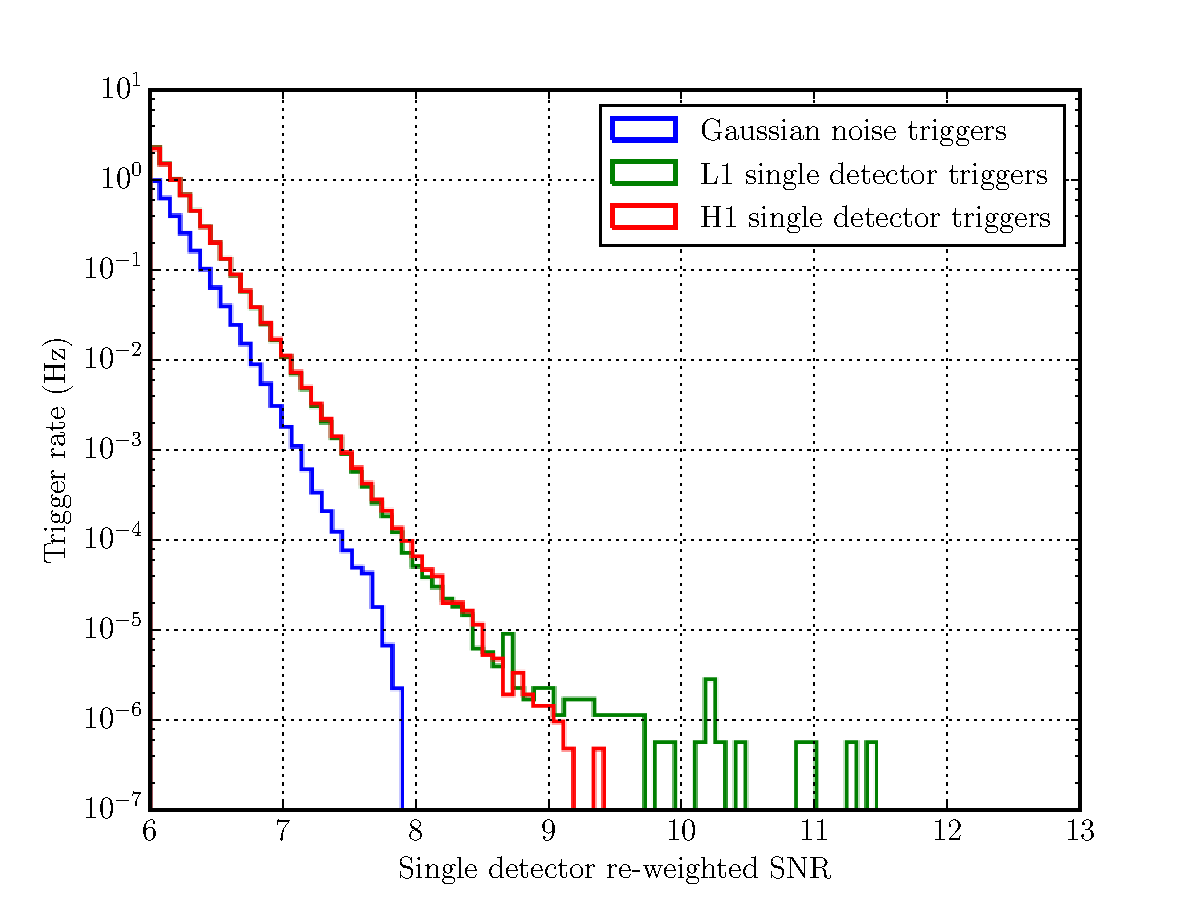
\includegraphics[width=0.8\textwidth]{figures/o1-cbc-dq-paper/H1-L1-Gaussian-newSNR-rate-hist}
  \caption[Rate histogram of PyCBC triggers vs. Gaussian noise]{A rate histogram %
           comparing the re-weighted SNR distribution in Gaussian %
           noise to that of real detector data. In Gaussian noise, the re-weighted %
           SNR distribution falls off before reaching $\hat{\rho} = 8$. %
           The distributions from real detector noise show extensive tails beyond %
           $\hat{\rho} = 8$ in addition to having an overall higher trigger rate.}
\label{fig:gaussian-rate}
\end{figure}



